%In this section we present $\pi$SOD-M, an MDD based methodology. 
$\pi$SOD-M provides an environment for building service compositions considering
their non-functional requirements. $\pi$SOD-M proposes the generation of a set of models at different abstraction levels, as well as transformations between these models.
$\pi$SOD-M includes non-functional specifications through
 four meta-models that extend PIM SOD-M meta-models (see Figure~\ref{fig:piSOD-M}): \textit{$\pi$-UseCase}, \textit{$\pi$-ServiceProcess}, \textit{$\pi$-ServiceCom\-po\-si\-tion} and \textit{$\pi$-PEWS}.

\begin{figure}[t]
\centering
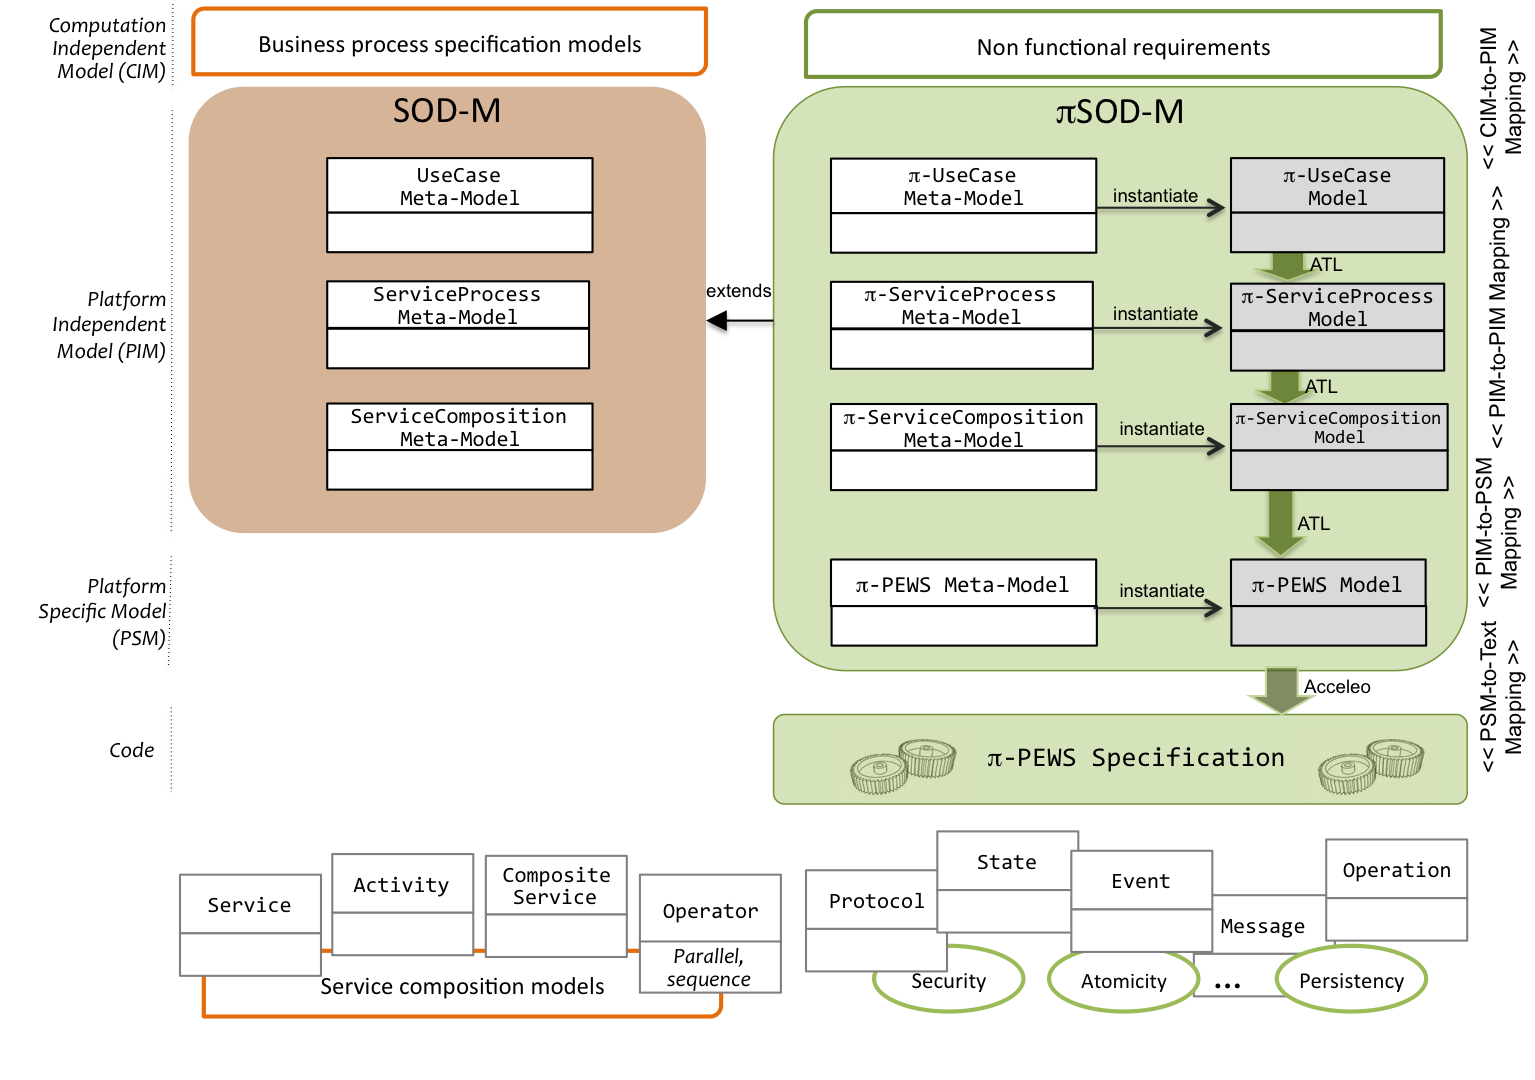
\includegraphics[width=1\textwidth]{figs/piSOD-M.png}
\caption{$\pi$SOD-M.}
\label{fig:piSOD-M}
\end{figure}
%
The \textit{$\pi$-UseCase} meta-model describes functional and non-functional requirements.
Non-functional requirements are defined as \textit{constraints} over processing and data. 
%
The \textit{$\pi$-ServiceProcess} meta-model defines the concept of \textit{service contract} to represent restrictions over data and actions that must be performed upon certain conditions. 
%
The \textit{$\pi$-ServiceProcess} meta-model gathers the constraints
described in the \textit{$\pi$-UseCase} model into contracts that are associated
with services. 
%
The \textit{$\pi$-ServiceComposition} meta-model provides the concept of \textit{Policy}~\cite{Espinosa-Oviedo2011a}
which put together contracts with similar non-functional requirements. 
For instance, security and privacy restrictions may be grouped into a security policy.
\textit{$\pi$-ServiceComposition} models can be refined into PSMs. Policies are associated to service operations and combine \textit{constraints} and \textit{reactive recovery actions}.
Constraints are restrictions that must be verified during the execution of the application. 
Failure to verify the constraints will trigger exceptions to execute their corresponding recovery actions.
An example of policy is the requirement of authentication for executing some of the system functions. 
The action associated to this policy may perform the authentication of the user.
%
The \textit{$\pi$-PEWS} meta-model is a PSM (see Figure~\ref{fig:piSOD-M}).
At the PSM level we have lower-level models that can be automatically translated into actual computer programs.
The \textit{$\pi$-PEWS} meta-model is the PSM adopted in this work.
\textit{$\pi$-PEWS} models are textual descriptions of service compositions that can be translated into PEWS~\cite{BHM06} %~\cite{BaCAM05,Placido2010LTPD} 
or BPEL~\cite{bpel03} code.
Although PEWS is our language of choice, other composition languages can be used as target.
%This can be accomplished by defining: \textit{(i)} a model-to-model transformation, from a \textit{$\pi$-ServiceComposition} model to the corresponding PSM, and \textit{(ii)} a model-to-text transformation, from the this PSM to the composition language.


%Note that $\pi$SOD-M extends the SOD-M meta-models by adding
%the concept of \textit{Policy}~\cite{Espinosa-Oviedo2011a}
%to represent non-functional requirements. 
%$\pi$SOD-M models represent both the functional aspects of the application as well as their non-functional behaviour. 


%In this context, we provide concepts at different levels of abstraction for expressing business rules of a process as policies (to implement existing NFP protocols).

%
%Similarly to SOD-M, our approach targets the construction of service-oriented applications that implement business processes.
Thus, $\pi$SOD-M proposes a development process based on the definition of models
(instances of the meta-models) and transformations between models.
There are two kinds of transformations:
Model-to-model transformations are used during the software process to refine the specification.
Model-to-text transformations are the last step of the process and generate code.

%%%BEGIN{Text Included by Placido Neto for Camera-Ready}%%%%%%
$\pi$SOD-M environment is built on the top of Eclipse. 
We also used the Eclipse Modelling Framework (EMF) to define, edit and handle
(meta)-models. 
To automate the transformation models we use ATL~\cite{atl_manual} and Acceleo~\cite{acceleo}.

In the next section we develop an example, to serve as a proof-of-concept.
The example will show the actual notation used for models. 





